\documentclass[11pt,a4paper]{article}
\usepackage[english]{babel}
\usepackage[utf8]{inputenc}
\usepackage{amsmath, amssymb}
\usepackage{graphicx}
\usepackage{caption}
\usepackage{float}
\usepackage[top=1in, left=1.25in, right=1.25in, bottom=.8in]{geometry}
\usepackage[numbered,framed]{matlab-prettifier}
\usepackage{filecontents}
\usepackage[T1]{fontenc}
\usepackage{bigfoot}
\usepackage{listings}

\numberwithin{equation}{subsection}
\newcommand{\eqname}[1]{\tag*{#1}}

\begin{filecontents*}{hw3.m}
%% Test 1
close all; clear all; clc
load cam1_1
load cam2_1
load cam3_1

% Compute the video frame size for each camera
[m1,n1]=size(vidFrames1_1(:,:,1,1));
[m2,n2]=size(vidFrames2_1(:,:,1,1));
[m3,n3]=size(vidFrames3_1(:,:,1,1));
% Compute video frame number for each camera
numFrames1=size(vidFrames1_1, 4);
numFrames2=size(vidFrames2_1, 4);
numFrames3=size(vidFrames3_1, 4);

% % Capture starting position of the paint can
% imshow(vidFrames1_1(:,:,1,1)); [iniY,iniX]=ginput(1);
% imshow(vidFrames2_1(:,:,1,1)); [iniY,iniX]=ginput(1); 
% imshow(vidFrames3_1(:,:,1,1)); [iniY,iniX]=ginput(1); 
% % Capture final position of the paint can
% imshow(vidFrames1_1(:,:,1,end)); [finY,finX]=ginput(1);
% imshow(vidFrames2_1(:,:,1,end)); [finY,finX]=ginput(1);
% imshow(vidFrames3_1(:,:,1,end)); [finY,finX]=ginput(1);

X1=[]; X2=[]; X3=[];
Y1=[]; Y2=[]; Y3=[];
% Convert each frame into a black and white image
% Then only keep the portion of paint can's movement
% figure(1)
% Camera 1
for j=1:numFrames1
    mov(j).cdata=vidFrames1_1(:,:,:,j);
    mov(j).colormap=[];
    X=frame2im(mov(j)); Xbw=rgb2gray(X);
    vidGray(:,:,j)=Xbw;
    Xbw(:,1:310)=0; Xbw(:,380:end)=0; % iniY : finY
    Xbw(1:210,:)=0; Xbw(420:end,:)=0; % iniX : finX
%     imshow(Xbw); drawnow
    [Xmax, Xind]=max(Xbw(:));
    [x1, y1]=ind2sub(size(Xbw), Xind);
    X1=[X1 x1]; Y1=[Y1 y1];
end
% Camera 2
for j=1:numFrames2
    mov(j).cdata=vidFrames2_1(:,:,:,j);
    mov(j).colormap=[];
    X=frame2im(mov(j)); Xbw=rgb2gray(X);
    vidGray(:,:,j)=Xbw;
    Xbw(:,1:250)=0; Xbw(:,340:end)=0; % iniY : finY
    Xbw(1:100,:)=0; Xbw(370:end,:)=0; % iniX : finX
%     imshow(Xbw); drawnow
    [Xmax, Xind]=max(Xbw(:));
    [x2, y2]=ind2sub(size(Xbw), Xind);
    X2=[X2 x2]; Y2=[Y2 y2];
end
% Camera 3
for j=1:numFrames3
    mov(j).cdata=vidFrames3_1(:,:,:,j);
    mov(j).colormap=[];
    X=frame2im(mov(j)); Xbw=rgb2gray(X);
    vidGray(:,:,j)=Xbw;
    Xbw(:,1:280)=0; Xbw(:,480:end)=0; % iniY : finY
    Xbw(1:240,:)=0; Xbw(340:end,:)=0; % iniX : finX
%     imshow(Xbw); drawnow
    [Xmax, Xind]=max(Xbw(:));
    [x3, y3]=ind2sub(size(Xbw), Xind);
    X3=[X3 x3]; Y3=[Y3 y3];
end

% Align data with equal length
minFrames=min([numFrames1, numFrames2, numFrames3]);
X1=X1(1:minFrames); X2=X2(1:minFrames); X3=X3(1:minFrames);
Y1=Y1(1:minFrames); Y2=Y2(1:minFrames); Y3=Y3(1:minFrames);
% Transform to frequency component using FFT
X1t = fft(X1); X2t = fft(X2); X3t = fft(X3);
Y1t = fft(Y1); Y2t = fft(Y2); Y3t = fft(Y3);
% Shannon window
X1t(10:end-10) = 0; X2t(10:end-10) = 0; X3t(10:end-10) = 0;
Y1t(10:end-10) = 0; Y2t(10:end-10) = 0; Y3t(10:end-10) = 0;
% Inverse transform to spatial signal
X1f = abs(ifft(X1t)); Y1f = abs(ifft(Y1t));
X2f = abs(ifft(X2t)); Y2f = abs(ifft(Y2t));
X3f = abs(ifft(X3t)); Y3f = abs(ifft(Y3t));

% Plot unfiltered X and Y spatial signal
figure(1)
subplot(3,1,1)
plot(1:minFrames, X1,'r',1:minFrames, Y1,'b', 'LineWidth',1.5)
xlabel('Frame (t)'); ylabel('Postion'); 
legend({'Y vs t','X vs t'},'Location','southeast','Fontsize',8)
title('(Case 1) Camera 1 mass motion over frame') 
set(gca, 'Xlim', [0 minFrames], 'Fontsize', 12)
subplot(3,1,2)
plot(1:minFrames, X2,'r',1:minFrames, Y2,'b','LineWidth',1.5)
xlabel('Frame (t)'); ylabel('Postion'); 
legend({'Y vs t','X vs t'},'Location','southeast','Fontsize',8)
title('(Case 1) Camera 2 mass motion over frame')
set(gca, 'Xlim', [0 minFrames], 'Fontsize', 12)
subplot(3,1,3)
plot(1:minFrames, X3,'r',1:minFrames, Y3,'b','LineWidth',1.5)
xlabel('Frame (t)'); ylabel('Postion'); 
legend({'Y vs t','X vs t'},'Location','southeast','Fontsize',8)
title('(Case 1) Camera 3 mass motion over frame')
set(gca, 'Xlim', [0 minFrames], 'Fontsize', 12)

% Plot filtered X and Y spatial signal
figure(2)
subplot(3,1,1)
plot(1:minFrames, X1f,'r',1:minFrames, Y1f,'b', 'LineWidth',1.5)
xlabel('Frame (t)'); ylabel('Postion'); 
legend({'Y vs t','X vs t'},'Location','southeast','Fontsize',8)
title('(Case 1) Camera 1 mass motion over frame (denosied)') 
set(gca, 'Xlim', [0 minFrames], 'Fontsize', 12)
subplot(3,1,2)
plot(1:minFrames, X2f,'r',1:minFrames, Y2f,'b','LineWidth',1.5)
xlabel('Frame (t)'); ylabel('Postion'); 
legend({'Y vs t','X vs t'},'Location','southeast','Fontsize',8)
title('(Case 1) Camera 2 mass motion over frame (denosied)')
set(gca, 'Xlim', [0 minFrames], 'Fontsize', 12)
subplot(3,1,3)
plot(1:minFrames, X3f,'r',1:minFrames, Y3f,'b','LineWidth',1.5)
xlabel('Frame (t)'); ylabel('Postion'); 
legend({'Y vs t','X vs t'},'Location','southeast','Fontsize',8)
title('(Case 1) Camera 3 mass motion over frame (denosied)')
set(gca, 'Xlim', [0 minFrames], 'Fontsize', 12)

% Performs PCA (SVD on covariance matrix)
X=[X1; Y1; X2; Y2; X3; Y3];
for k=1:minFrames
    X(:,k)=X(:,k)-mean(X,2);
end
[U, S, V]=svd(cov(X));
sig=diag(S);

% Plot PCA results
figure(3)
plot((sig/sum(sig))*100, 'ro--', 'LineWidth', 1.5), axis([1 6 0 100])
xlabel('Modes'); ylabel('% of Energy'); 
title('(Case 1) Energy percentage captured by each mode after SVD')
set(gca, 'Fontsize', 12)

% Compute energy of first four modes
energy1=sig(1)/sum(sig);
energy2=sig(1:2)/sum(sig);
energy3=sig(1:3)/sum(sig);
energy4=sig(1:4)/sum(sig);
\end{filecontents*}
\let\ph\mlplaceholder % shorter macro
\lstMakeShortInline"
\lstset{
  style              = Matlab-editor,
  basicstyle         = \mlttfamily,
  escapechar         = ",
  mlshowsectionrules = true,
}

\title{Amath 482 Winter 2019 \\
HW3: PCA}
\author{Wenrui Yuan}
\date{\today}

\begin{document}
\maketitle

\begin{abstract}
	This report studies movements of a oscillating mass system by applying Principle Component Analysis (PCA) on videos taken by three different cameras. As a special case of the Singular Value Decomposition (SVD) method, PCA will help us to remove redundant information. We will also compare different movements to understand how they effect PCA results.
\end{abstract}


\section{Introduction and Overview}
	Principle Component Analysis (PCA)or Proper Orthogonal Decomposition (POD) is a statistical method that applies orthogonal transformation to convert a set of data with correlated variables into one with linearly uncorrelated variables.\cite{pca}\\
	This report will study four test, each with three cameras filming various movements of a paint can. The first test is an ideal case which almost recreate the simple harmonic motion. The second case will be a similar one with some camera shakes (noises). We will face more complicated movements by adding horizontal displacement (i.e. the single pendulum movement) in test 3 and horizontal displacement as well as rotations in test 4. After studying these cases, we will be able to apply PCA and compare results with the actual movements shown in the videos and determine how well can PCA perform under various conditions.


\section{Theoretical Background}
\subsection{Singular Value Decomposition}
The Singular Value Decomposition is a factorization of real of complex valued matrix that gives us information on scalings and rotations of the matrix. Suppose $A \text{ is a } m\times n \text{ matrix}$, the SVD of $A$ generally has the form \cite{svd}
\begin{equation}
A=U\Sigma V^*
\end{equation}
where $U\in \mathbb{C}^{m\times m}$ and $V\in \mathbb{C}^{n\times n}$ is unitary (orthogonal), $\Sigma\in \mathbb{R}^{m\times n}$ is diagonal and $V^*$ is just the conjugate transpose of $V$. Note that every matrix has SVD, and the singular values $\left\{ \sigma_{j}\right\}$ are uniquely determined, which is very helpful in low-dimensional approximation\cite{582}.

\subsection{Principal Component Analysis}
PCA is a key application of SVD using the idea of covariance. In general, suppose we have m modes that each takes n measurements, which can be written into a matrix $X\in\mathbb{C}^{m\times n}$. However, as these data contains some noises and irrelevant information, we can eliminate redundant measurements by computing the covariance of $X$.\\
Recall that given two sets of measurement $a=[a_1, a_2, a_3, \cdots] \text{ and } b=[b_1, b_2, b_3, \cdots]$, the covariance between $a$ and $b$ is defined as \cite{582}
\begin{equation}
\sigma^{2}_{ab}=\frac{1}{n-1}ab^T
\end{equation}
Now since we have multiple ``sets'' of measurement, the covariance of $X$ is given by \cite{582}
\begin{equation}
C_X=\frac{1}{n-1}XX^T
\end{equation}
where $C_X$ is a $m\times m$ symmetric matrix. Finally, we want to diagonalize the covariance matrix to find an ideal basis in which $C_X$ is diagonal (i.e. no redundant information).



\section{Algorithm Implementation and Development}
Although there are multiple cases to be studied in this report, they all follow the same principle in terms of algorithm development with slight variations. Thus only the general idea and approach will be covered in this section.
\begin{itemize}
\item \textbf{Load data and compute frame numbers}
\item \textbf{Determine portion size}\\
Use \textbf{ginput(1)} to manually locate the starting postion as well as the ending coordinate. This helps us to select how much information to keep in later steps.
\item \textbf{Convert each picture frame into a black and white one}\\
As aforementioned, we are not interested in the color as there is a light on the paint can, but in tracking movements of the light (strongest signal).
\item \textbf{Isolate motion of the paint can}\\
This can be accomplished by set all data describing other parts on the image of each frame to zero. This is necessary because ambient lights in each frame make it hard to locate the light on the paint can.
\item \textbf{Find the strongest signal(light) of each frame}\\
As we know that the light gives the strongest signal (attains maximum). Compute the maximum and its index of each frame using the \texttt{max} and corresponding subscripts using \texttt{ind2sub}.
\item \textbf{Assign same size to arrays}\\
As the number of frames for each camera is different, the positional data we get from previous step are not of equal length. Thus we must set the minimum frame numbers among all three cameras to be the maximum number of samples.
\item \textbf{Apply Shannon window to the data}\\
Notice that the data is noisy even for the ideal case. Therefore we first \texttt{fft} the positional data (\texttt{X \text{and} \texttt{Y}}) and use a Shannon Window to filter out noisy frequencies before transforming back to signals using \texttt{ifft}
\item \textbf{Form \texttt{X Y} positions for each camera into a matrix}\\
We have already forced positional data from each camera to have the same length, the matrix is constructed by stacking these vectors
\item \textbf{Performs PCA to the stacked matrix}\\
Recall that we need to compute "svd" of the covariance matrix and diagonalize it to derive the principle components. 

\end{itemize}


\section{Computational Results}
\subsection{Test 1: Ideal case}
\begin{figure}[H]
\begin{center}
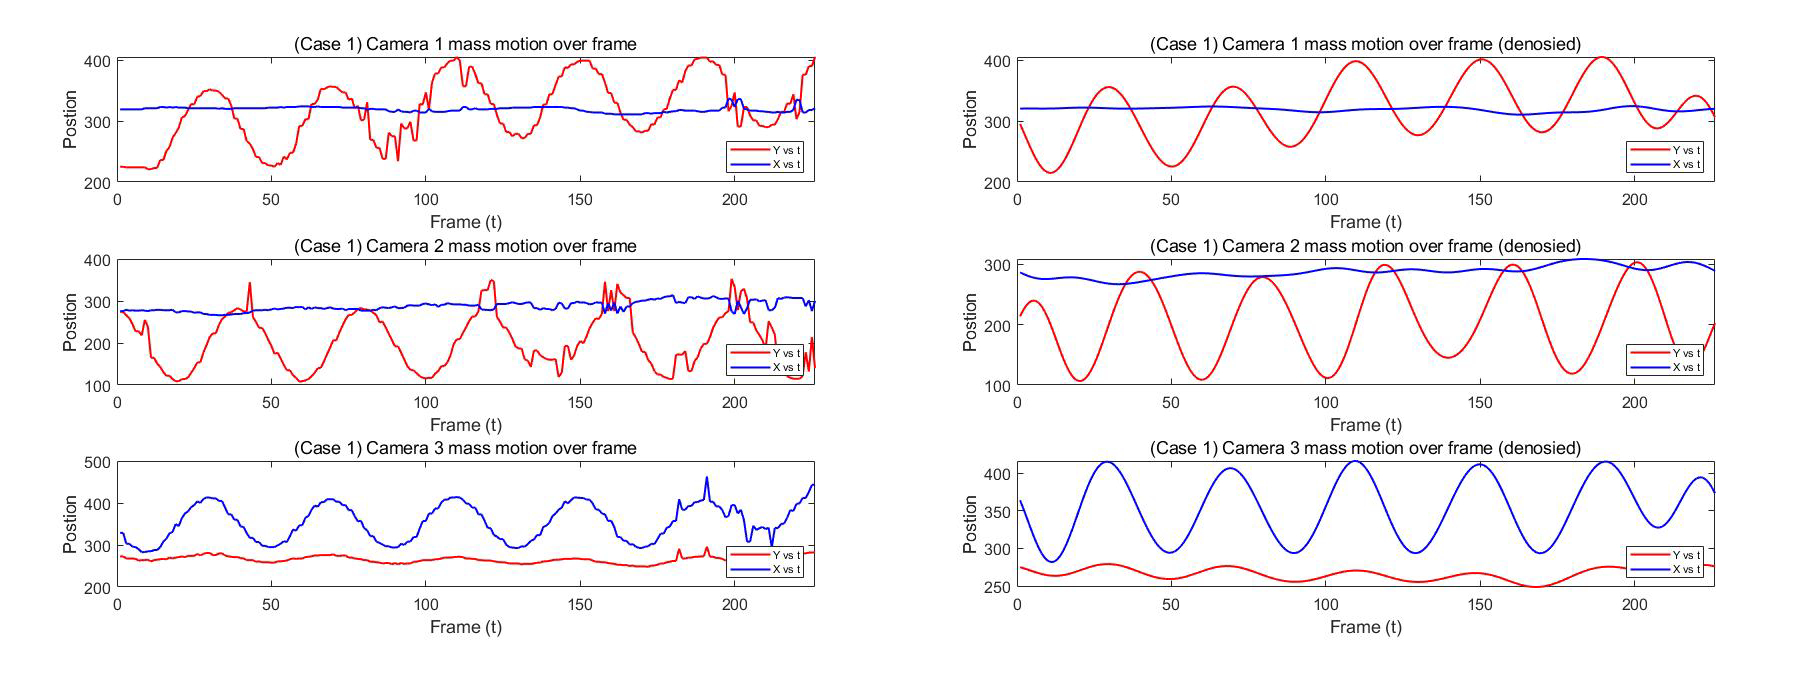
\includegraphics[scale=0.20]{f1.jpg}
\caption{Unfiltered (left) and denoised (right) X-Y position of can over frame for case 1}
\end{center}
\end{figure}
We start with the ideal case, where the paint can was released at certain height to simulate a simple harmonic motion. Notice that although all videos have the size \texttt{640*480}, data converted from them are 4D matrices in which the part of first two dimensions is of size \texttt{480*640}. Then, motion occurred along x-axis was actually recorded on the y-axis. We can clearly observe that the variation of Y-positions describe the simple harmonic motion just as expected. Now, as camera 3 was flipped by 90 degrees, Y-coordinates are actually the X-coordinates in the real world. There are differences between filtered and unfiltered spatial signals, but since this case is an ideal experiment, the variation is not noticeable.
\begin{figure}[H]
\begin{center}
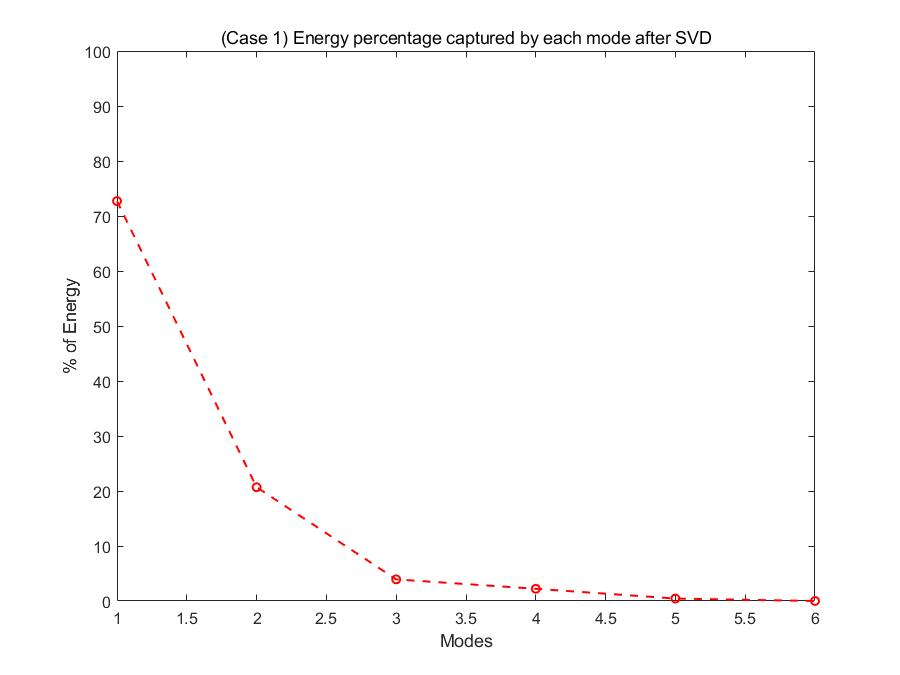
\includegraphics[scale=0.20]{f2.jpg}
\caption{Percentage of energy captured by each mode computed by SVD for case 1}
\end{center}
\end{figure}
We observe from figure 2 that the first mode captures nearly 73\% of energy and if we combine the following one, the first modes devote nearly 94\% of energy. This suggests that we can almost recreate the dynamics of the paint can with first two modes.

\subsection{Test 2: Noisy case}
\begin{figure}[H]
\begin{center}
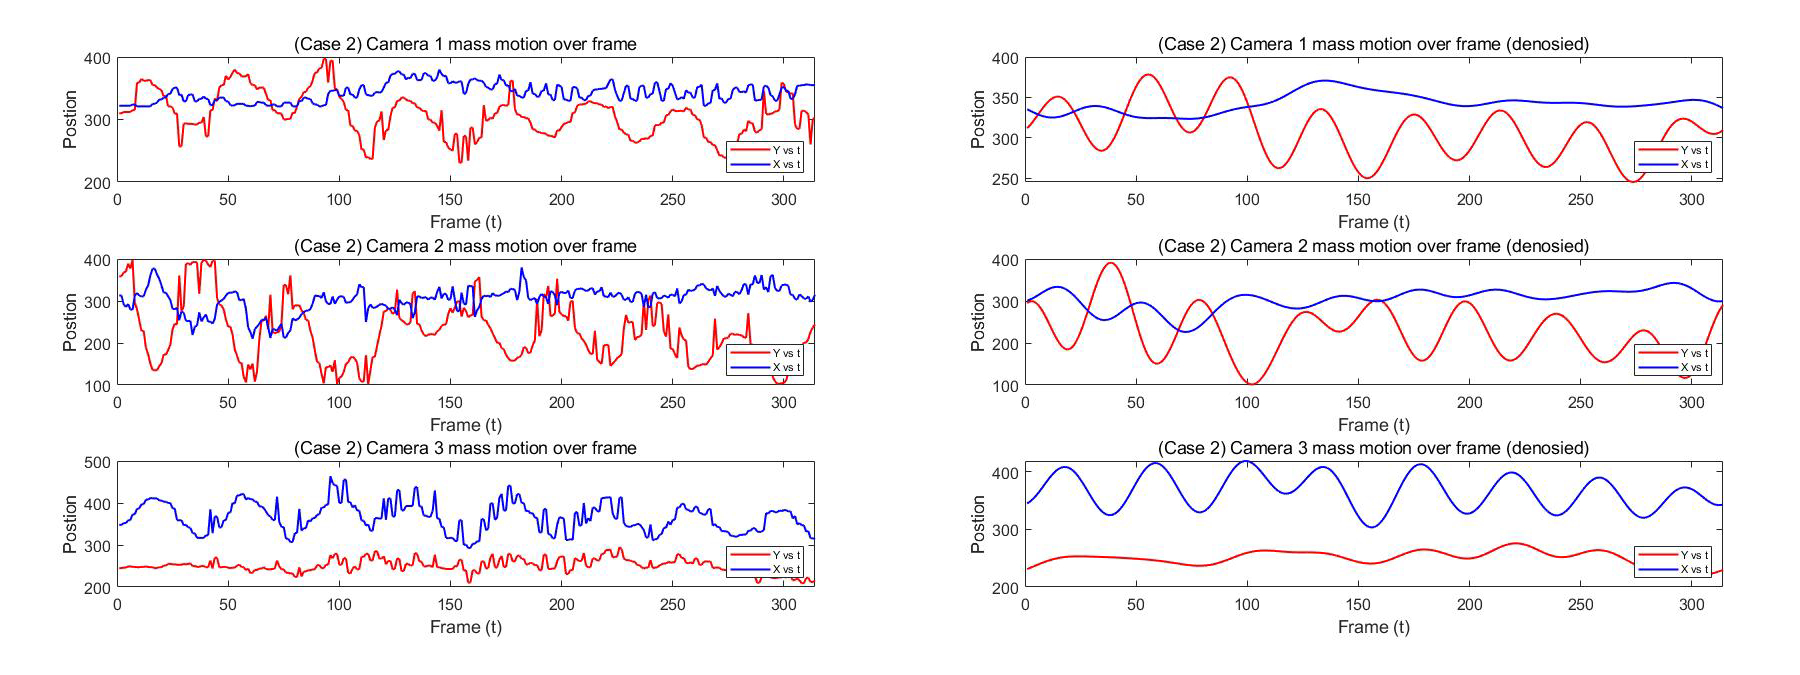
\includegraphics[scale=0.20]{f3.jpg}
\caption{Unfiltered (left) and denoised (right) X-Y position of can over frame for case 2}
\end{center}
\end{figure}
As soon as we moved to test 2, there are many noticeable spikes in both X and Y direction shown in left of Figure 3. Compared with Figure 1, although the motion is almost the same, camera tilting creates lots of noises.
\begin{figure}[H]
\begin{center}
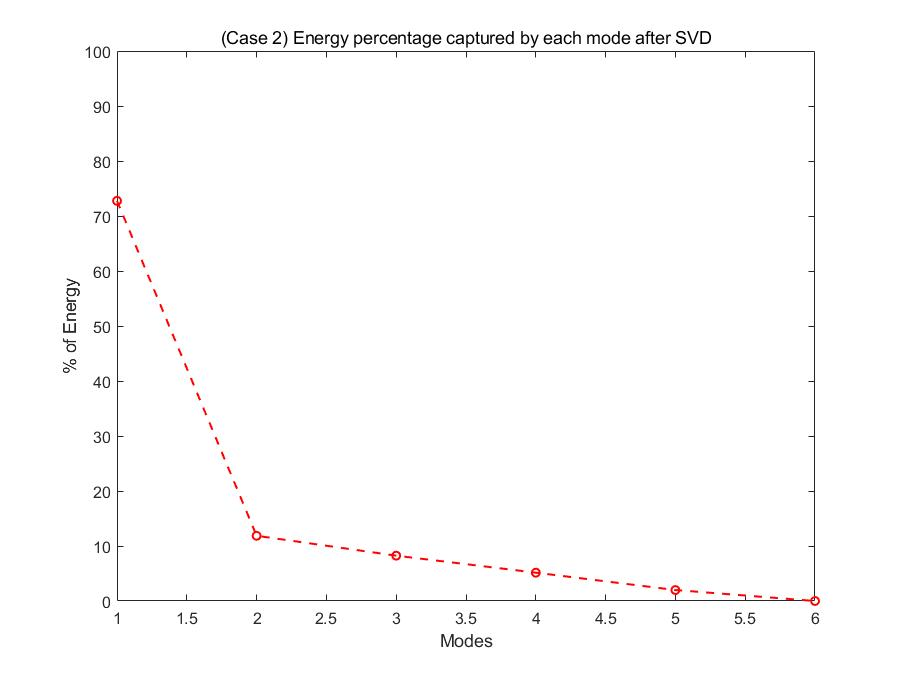
\includegraphics[scale=0.20]{f4.jpg}
\caption{Percentage of energy captured by each mode computed by SVD for case 2}
\end{center}
\end{figure}
Surprisingly, figure 4 shows that the first two modes obtain 84\% of total energy while the first four modes capture 98\%. We can see that noise does effect the amount of energy captured by each mode but the result is still helpful for motion tracking.

\subsection{Test 3: Horizontal displacement}
\begin{figure}[H]
\begin{center}
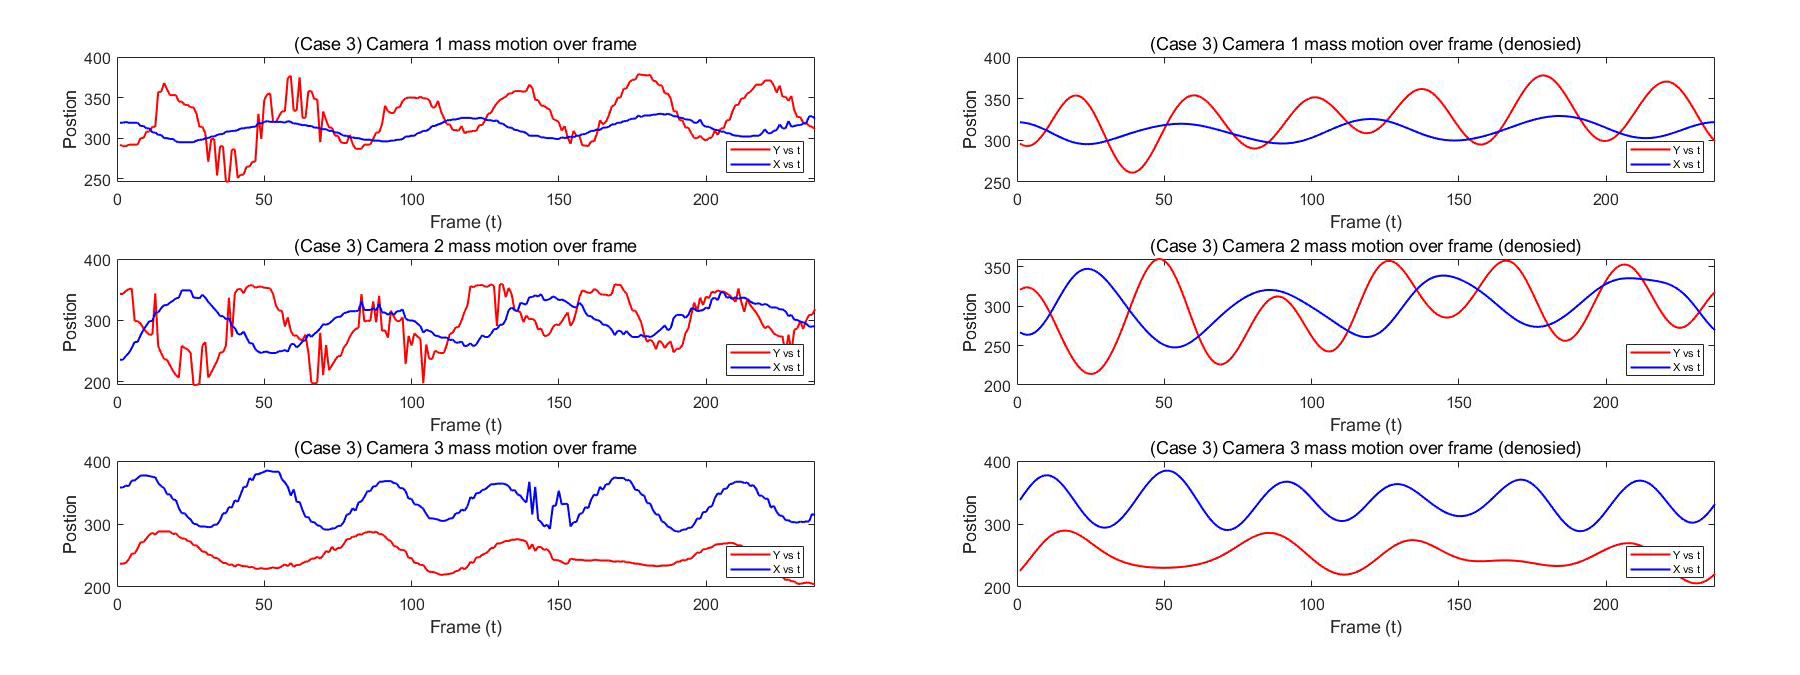
\includegraphics[scale=0.20]{f5.jpg}
\caption{Unfiltered (left) and denoised (right) X-Y position of can over frame for case 3}
\end{center}
\end{figure}
The motion gets more complex in the third case where the paint can was also performing the motion of a singular pendulum while doing the simple harmonic motion. In this case, we expect a slight X position variation and the variation in the Y direction to be still noticeably big. As we can see, motion recorded by camera 3 better indicates the actual motion of paint can as there are less noises.
\begin{figure}[H]
\begin{center}
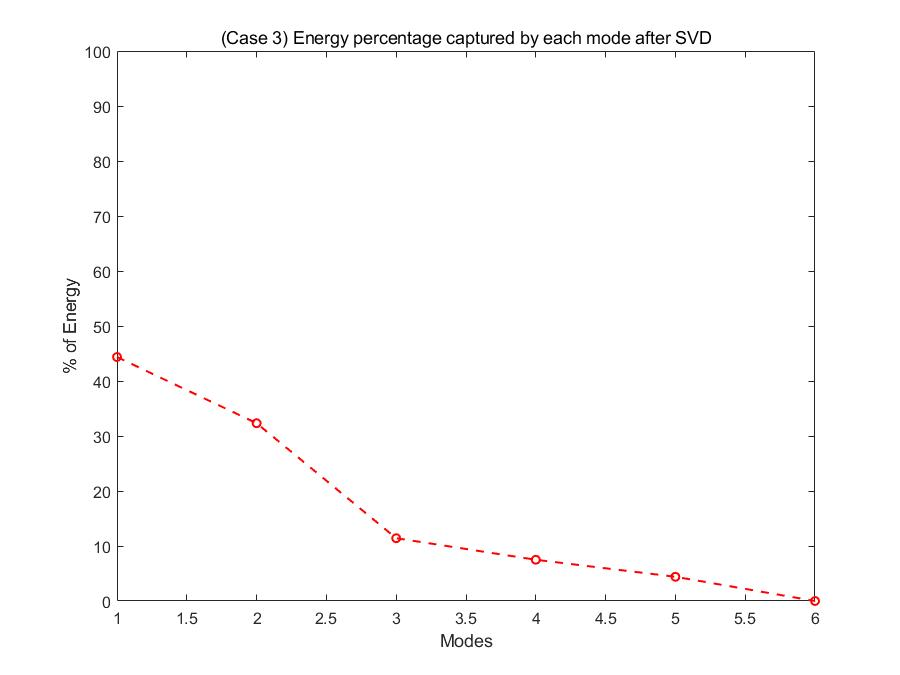
\includegraphics[scale=0.20]{f6.jpg}
\caption{Percentage of energy captured by each mode computed by SVD for case 3}
\end{center}
\end{figure}
However, we know from figure 6 that percentage of energy captured by first two modes are not so big compared with previous two cases. Unlike any of previous cases, the first mode captureed less than 50\% of energy and first two modes combined commits only 77\% of energy, which is still reasonable as we see there as the paint can actually moves in 3D and there was slight displacement along the Z-axis. This suggests that PCA does not perform quite well due to small covariances and deviation in actual movements.


\subsection{Test 4: Horizontal displacement and rotation}
\begin{figure}[H]
\begin{center}
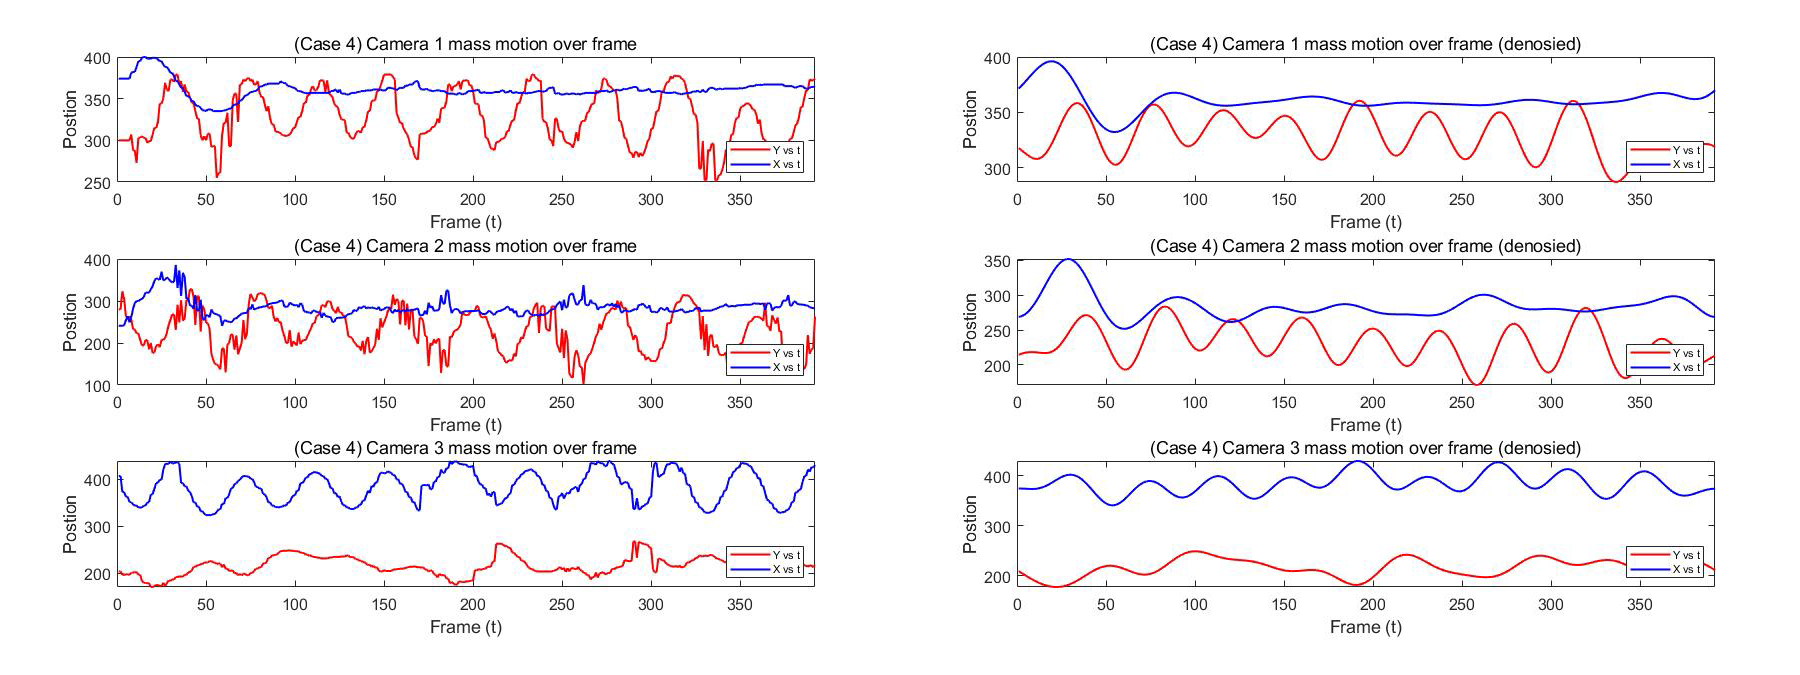
\includegraphics[scale=0.20]{f7.jpg}
\caption{Unfiltered (left) and denoised (right) X-Y position of can over frame for case 4}
\end{center}
\end{figure}
The paint can was set to rotate and then release in this case. The ``big swing'' in first few seconds was shown by plots of camera 1 and 2, possibly due to the initial rotational acceleration.
\begin{figure}[H]
\begin{center}
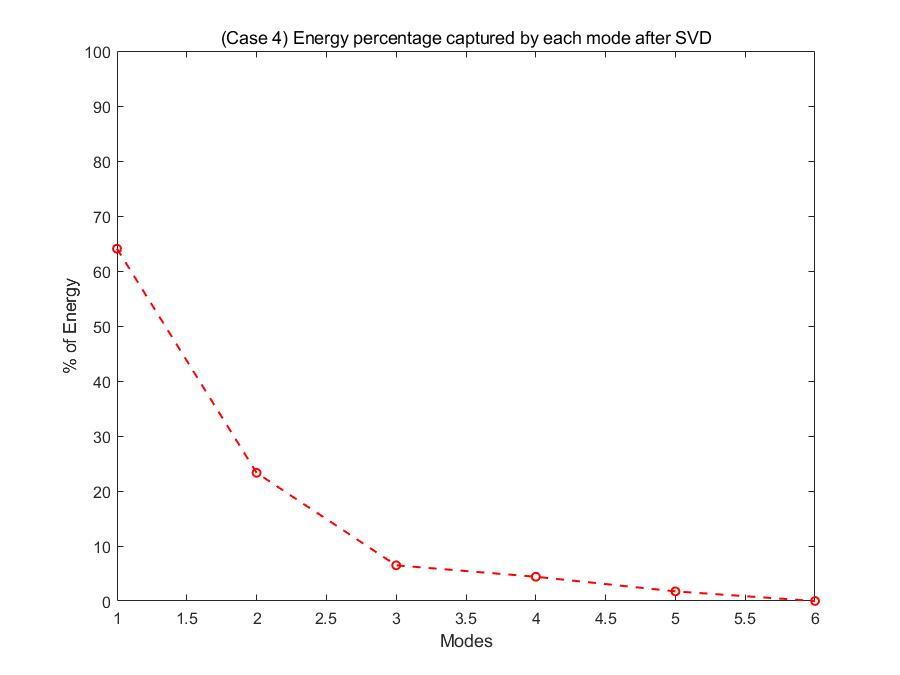
\includegraphics[scale=0.20]{f8.jpg}
\caption{Percentage of energy captured by each mode computed by SVD for case 4}
\end{center}
\end{figure}
Now we observe from figure 8 that the first two modes capture 87\% of energy, which is better than ones in the previous test possibly due to less horizontal displacement caused by the rotation. Moreover, as the sum of percentage of energy for the first four modes is 98\%, meaning that we will need two cameras to obtain more accurate approximation.



\section{Summary and Conclusions}
We observe that if the motion was more simple(as in Test 1 and 2), first two modes can capture enough energy to describe the motion, which means one camera is enough for our principle component analysis. Meanwhile, although camera shakes all the time, PCA results is quite assuring that first two modes did not lose much accuracy in terms of motion tracking. This suggests that PCA will be able to handle noisy signals if data is relatively simple (i.e.small variation).\\
For case 3 and 4, we do expect results to be less accurate as the motions get more complex, yet PCA of case 4 implies that rotation over time does attenuate horizontal displacement and therefore the motion tracking is more accurate.\\
Generally speaking, PCA is very practically useful in approximating simple movements (i.e. motion along one direction) and lose a lot of accuracy when the movements gets more complex. Moreover, noise does have effect on the analysis but the performance will get better if more modes are deployed.


\begin{thebibliography}{11}
	\bibitem{582}
	J. Nathan Kutz. 2013.
	\textit{Data-Driven Modeling \& Scientific Computation}. p. 53-74
	
	\bibitem{mtlb}
	\textit{Matlab Documentation. Mathworks}; [2019 Feb 25]. \\https://www.mathworks.com/help/index.html

	\bibitem{pca}
	\textit{Singular Value Decomposition. Wikipedia}; [2019 Feb 25]. \\https://www.en.wikipedia.org/wiki/Singular\_Value\_Decomposition

	\bibitem{svd}
	\textit{Principle Component Analysis. Wikipedia}; [2019 Feb 25]. \\https://www.en.wikipedia.org/wiki/Principle\_Component\_Analysis
\end{thebibliography}


\section*{Appendix A: MATLAB functions used}
	\begin{itemize}
		\item \texttt{strcat}\\
		Concatenate strings horizontally
		\item \texttt{dir}\\
		List folder contents
		\item \texttt{imread}\\
		Read the image from the file specified by "filename"
		\item \texttt{repmat}\\
		"B = repmat(A,r1,... ,""rN)" specifies a list of scalars, "r1,..,rN", that describes how copies of "A" are arranged in each dimension
		\item \texttt{fft}\\
		Compute the 1-D Fourier transform using FFT algorithm
		\item \texttt{ifft}\\
		\texttt{X = ifft(Y)} computes the inverse Fourier transform of Y using FFT algorithm
		\item \texttt{ind2sub}\\
\texttt{[X, Y] = ind2sub(siz,IND)} returns subscript arrays \texttt{X} and \texttt{Y} with given indices \texttt{IND} of a matrix size \texttt{siz}
		\item \texttt{svd}\\
		\texttt{[U,S,V] = svd(A)} performs a singular value decomposition of matrix \texttt{A}, such that \texttt{A = U*S*V'}
		\item \texttt{cov}\\
		\texttt{C = cov(A)} returns the covariance matrix \texttt{C}.		
		\item \texttt{diag}\\
		\texttt{x = diag(A)} returns a column vector of the main diagonal elements of A.

	\end{itemize}


\section*{Appendix B: MATLAB codes}
All four tests share similar code with only a few changes in variable values. Thus only code for the first test will be included due to page restriction.
\lstinputlisting{hw3.m}




\end{document}
